\chapter{Dynamique de Friedmann : matière, rayonnement et énergie du vide}

\lectureoverview{La cinématique d’un univers en expansion peut se résumer en une ligne : les distances physiques croissent avec un facteur d’échelle \(a(t)\). Il s’agit maintenant de déterminer cette fonction. Nous retrouverons l’équation de Friedmann de l’espace plat à partir de la conservation newtonienne de l’énergie, la résoudrons d’abord pour la matière ordinaire, puis verrons pourquoi le rayonnement et l’énergie du vide conduisent à des histoires cosmiques entièrement différentes.}

\section{La géométrie à expliquer}

À un instant cosmique donné, l’Univers à grande échelle paraît homogène et isotrope. Les galaxies, les amas et les superamas sont bien des structures réelles, mais à des échelles de centaines de millions ou de milliards d’années-lumière, leur répartition devient remarquablement uniforme. Cette régularité empirique est appelée principe cosmologique. Ce nom n’en fait pas un théorème ; le principe tire sa force de l’observation.

Il existe un second fait empirique. Dans les limites de la précision actuelle, les grands triangles spatiaux se comportent comme des triangles euclidiens. L’analogie avec l’arpentage d’un terrain de football est utile. Si des lignes bien tendues forment des triangles dont la somme des angles vaut \(180^\circ\), cela ne prouve pas que la Terre est globalement plate. Cela montre que son rayon de courbure est grand par rapport au terrain. L’arpentage cosmique suit la même logique : l’espace peut avoir un très grand rayon de courbure, mais, dans la région observable, il est bien approximé par un espace plat.

La géométrie de référence est l’espace-temps de Minkowski,
\begin{equation}
  d\tau^2=dt^2-\left(dx^2+dy^2+dz^2\right).
  \label{eq:l09-minkowski}
\end{equation}
Le crochet désigne simplement l’élément de distance euclidienne en trois dimensions. En relativité générale, en revanche, les coefficients des différentielles de coordonnées sont des champs. Ils peuvent varier avec la position et le temps, et des termes croisés peuvent aussi apparaître. Ces coefficients métriques sont les successeurs relativistes du champ gravitationnel newtonien.

\begin{figure}[H]
  \centering
  \includegraphics[width=0.72\textwidth]{lecture_09_figure_01.png}
  \caption{L’élément de temps propre de Minkowski écrit au début du cours. Référentiel source à 00:01:50.}
  \label{fig:l09-minkowski-board}
\end{figure}

Pour un univers en expansion spatialement plat, l’homogénéité et l’isotropie ne laissent qu’un facteur d’échelle dépendant du temps :
\begin{equation}
  d\tau^2=dt^2-a^2(t)\left(dx^2+dy^2+dz^2\right).
  \label{eq:l09-flat-frw}
\end{equation}
Nous utilisons des unités dans lesquelles \(c=1\), de sorte que le temps et la longueur ont les mêmes dimensions. Deux conventions cohérentes sont possibles. On peut donner à \(x,y,z\) les dimensions d’une longueur et prendre \(a\) sans dimension, ou traiter \(x,y,z\) comme des coordonnées sans dimension et laisser \(a\) porter les dimensions d’une longueur. Le cours adopte la seconde convention, car elle rend manifeste le sens physique de \(a(t)\).

\begin{figure}[H]
  \centering
  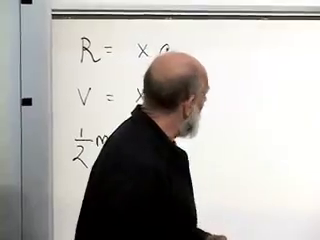
\includegraphics[width=0.72\textwidth]{lecture_09_figure_02.png}
  \caption{La métrique plate en expansion, où le facteur d’échelle multiplie l’élément de ligne spatiale euclidien. Référentiel source à 00:09:12.}
  \label{fig:l09-expanding-metric-board}
\end{figure}

Imaginons des coordonnées peintes sur une feuille de caoutchouc. Les repères de coordonnées restent attachés à la feuille tandis que la distance physique entre eux augmente. Ainsi, une différence de coordonnées telle que « de \(x=0\) à \(x=1\) » n’est qu’une paire de repères. La distance représentée par cet intervalle est \(a(t)\). Trouver l’équation qui régit ce facteur d’échelle est le problème dynamique du cours.

\section{Géométries spatiales fermées, plates et ouvertes}

La platitude est une simplification observationnelle, et non une conséquence de l’homogénéité. Il existe trois géométries spatiales homogènes et isotropes : à courbure positive, nulle et négative. Pour comprendre le cas positif, il est utile de préciser la dimension.

Le lieu
\begin{equation}
  X_1^2+X_2^2=R^2
\end{equation}
est un cercle, ou une sphère de dimension un \(S^1\). Son intérieur rempli est un disque, également appelé boule de dimension deux. En ajoutant une coordonnée d’immersion, on obtient
\begin{equation}
  X_1^2+X_2^2+X_3^2=R^2,
\end{equation}
la sphère ordinaire de dimension deux \(S^2\). En ajoutant une quatrième coordonnée d’immersion, on obtient
\begin{equation}
  X_1^2+X_2^2+X_3^2+X_4^2=R^2,
  \label{eq:l09-three-sphere}
\end{equation}
une sphère de dimension trois \(S^3\), qui est elle-même un espace à trois dimensions. Nous ne pouvons pas nous représenter son immersion en quatre dimensions, mais sa géométrie intrinsèque n’a pas besoin de cette immersion pour exister.

\begin{figure}[H]
  \centering
  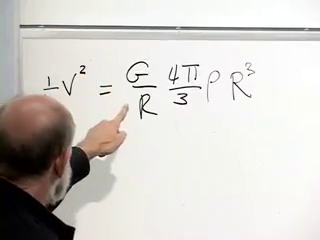
\includegraphics[width=0.72\textwidth]{lecture_09_figure_03.png}
  \caption{L’équation d’immersion utilisée pour introduire la sphère de dimension trois. Référentiel source à 00:16:40.}
  \label{fig:l09-three-sphere-board}
\end{figure}

Tous les points d’une sphère idéale sont géométriquement équivalents, et toutes les directions en un point le sont également. Une sphère est donc à la fois homogène et isotrope. Si son rayon est multiplié par \(a(t)\), tout l’espace se dilate ou se contracte sans qu’un centre soit privilégié sur la sphère. Remonter le cours du temps dans un tel univers ne ramène pas toute la matière à un lieu particulier dans un vide extérieur. L’espace entier devient petit, si bien que chaque paire de points se rapproche. Le Big Bang n’est pas une explosion à partir d’un point de l’espace.

Sur une sphère à courbure positive, la somme des angles d’un triangle géodésique est supérieure à \(180^\circ\). Dans un triangle plat, elle vaut exactement \(180^\circ\). Dans une géométrie homogène à courbure négative, imparfaitement représentée par une selle, elle est inférieure à \(180^\circ\). Ces tests intrinsèques distinguent les trois cas.

\begin{figure}[H]
  \centering
  \includegraphics[width=0.72\textwidth]{lecture_09_figure_07.png}
  \caption{Courbures positive, nulle et négative, représentées par les formes caractéristiques de leurs triangles. Référentiel source à 00:37:30.}
  \label{fig:l09-curvature-board}
\end{figure}

Une métrique parfaitement plate localement ne prouve pas à elle seule que l’espace est topologiquement infini. Des topologies plates compactes sont mathématiquement possibles, même si le cours adopte le modèle euclidien infini le plus simple.
\editorialnote{Cette réserve sur la topologie globale n’est nécessaire pour aucune des dynamiques locales qui suivent.}

\section{Repères comobiles et loi de Hubble}

Revenons à la feuille plate en expansion et traçons-y un quadrillage de coordonnées. En coordonnées comobiles, la grille se dilate avec le flux de matière à grande échelle. Une galaxie, ou plus précisément un amas de galaxies défini à une échelle suffisamment grossière, conserve un repère de coordonnées approximativement fixe, même si sa distance physique à un autre objet comobile varie.

\begin{figure}[H]
  \centering
  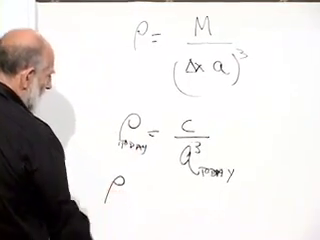
\includegraphics[width=0.72\textwidth]{lecture_09_figure_04.png}
  \caption{Un quadrillage de coordonnées entraîné par une feuille spatiale en expansion. Référentiel source à 00:22:20.}
  \label{fig:l09-comoving-grid-board}
\end{figure}

Pour deux objets séparés le long de l’axe \(x\) par un intervalle comobile fixe \(\Delta x\), leur distance physique est
\begin{equation}
  D(t)=a(t)\,\Delta x.
  \label{eq:l09-physical-distance}
\end{equation}
En dérivant par rapport au temps à \(\Delta x\) constant, on obtient
\begin{equation}
  v(t)=\dot a(t)\,\Delta x
      =\frac{\dot a(t)}{a(t)}D(t).
\end{equation}
En définissant
\begin{equation}
  H(t)\equiv\frac{\dot a(t)}{a(t)},
  \label{eq:l09-hubble-parameter}
\end{equation}
on obtient la loi de Hubble,
\begin{equation}
  v=H(t)D.
  \label{eq:l09-hubble-law}
\end{equation}
Dans l’expression « constante de Hubble », le mot « constante » signifie qu’elle est la même dans tout l’espace à un instant cosmique donné. Cela ne signifie pas qu’elle reste constante au cours de l’histoire cosmique.

\begin{figure}[H]
  \centering
  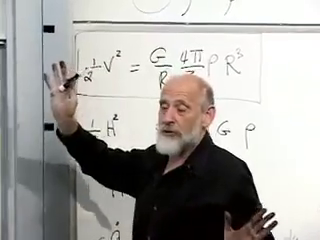
\includegraphics[width=0.72\textwidth]{lecture_09_figure_05.png}
  \caption{La dérivation au tableau \(D=a\Delta x\),
  \(v=(\dot a/a)D=HD\). Référentiel source à 00:26:40.}
  \label{fig:l09-hubble-board}
\end{figure}

\begin{classroomqa}
\audiencequestion{Si l’on observe une galaxie lointaine à une époque antérieure, son paramètre de Hubble inféré devrait-il vraiment être égal à la valeur mesurée aujourd’hui dans notre voisinage ?}
\lecturerresponse{Seulement si le temps rétrospectif est faible devant l’âge de l’Univers. Sur des distances modérées, \(H(t)\) varie assez peu pour qu’une seule valeur soit utile. À des distances véritablement cosmologiques, nous observons des époques plus anciennes, et il faut tenir compte de la dépendance temporelle de \(a\) et de \(H\). C’est l’une des raisons pour lesquelles nous avons besoin d’une équation dynamique pour le facteur d’échelle.}
\end{classroomqa}

\section{Rayons lumineux nuls dans un système de coordonnées en expansion}

\begin{classroomqa}
\audiencequestion{Le facteur d’échelle affecte-t-il la propagation de la lumière entre des galaxies lointaines ?}
\lecturerresponse{Un rayon lumineux suit une trajectoire nulle, donc \(d\tau=0\). Pour un rayon se propageant le long de l’axe positif \(x\), on a \(dy=dz=0\), et la métrique en expansion donne
\begin{align}
  0&=dt^2-a^2(t)dx^2,
  &dt&=a(t)dx,\notag\\
  &&\frac{dx}{dt}&=\frac{1}{a(t)}.
  \label{eq:l09-null-ray}
\end{align}
La vitesse coordonnée diminue à mesure que \(a(t)\) augmente, mais la vitesse physique locale de la lumière reste égale à \(c=1\). Un intervalle de coordonnées fixe représente une distance physique croissante.}
\end{classroomqa}

\begin{figure}[H]
  \centering
  \includegraphics[width=0.72\textwidth]{lecture_09_figure_06.png}
  \caption{La condition de nullité et \(dt=a(t)dx\) pour la propagation radiale de la lumière. Référentiel source à 00:30:54.}
  \label{fig:l09-null-board}
\end{figure}

On pourrait choisir des coordonnées dans lesquelles ce même fait se formulerait ainsi : « la lumière ralentit à mesure qu’on s’éloigne », mais les longueurs et les horloges prendraient alors des descriptions tout aussi peu commodes. Le langage de l’espace en expansion est plus clair, car il préserve l’énoncé local selon lequel tout observateur en chute libre mesure la même vitesse de la lumière.

\begin{classroomqa}
\audiencequestion{Existe-t-il des indices montrant que la propagation locale de la lumière et la physique atomique sont les mêmes dans les galaxies lointaines ?}
\lecturerresponse{Seules les comparaisons sans dimension ont un sens opérationnel. Prenons la taille d’un atome comme unité de longueur et une période atomique ou nucléaire comme unité de temps, puis demandons combien de telles périodes la lumière met à parcourir la longueur choisie. Les observations spectrales étayent l’affirmation selon laquelle ces rapports sans dimension sont les mêmes dans des régions lointaines. Les indices sont indirects, mais c’est précisément par ce type de comparaison que l’on vérifie l’uniformité des lois locales.}
\end{classroomqa}

Lorsque l’Univers observable était extrêmement petit, la lumière pouvait traverser rapidement une région physique donnée, si l’on mesure le temps en temps de traversée de la lumière correspondant à cette région. Cela ne signifie pas que \(c\) était différent. Cela signifie que la région elle-même était petite.

\section{Une sphère newtonienne dans l’Univers}

Passons maintenant de la cinématique à la dynamique. Plaçons-nous à l’origine et traçons une sphère assez grande pour contenir de nombreuses galaxies et de nombreux amas. Choisissons une galaxie sur sa frontière. Dans un univers homogène, la distribution de masse est sphériquement symétrique autour de nous, et le théorème des coquilles de Newton donne deux résultats essentiels :
\begin{enumerate}
  \item toute la matière distribuée sphériquement à l’extérieur du rayon choisi exerce une force newtonienne nette nulle sur la galaxie située à la frontière ;
  \item toute la matière contenue dans la sphère agit, pour ce mouvement radial, comme si elle était concentrée au centre.
\end{enumerate}
Nous choisissons un référentiel dans lequel nous sommes au repos ; les vitesses et les accélérations de l’argument qui suit sont donc mesurées par rapport à nous.

\begin{figure}[H]
  \centering
  \includegraphics[width=0.72\textwidth]{lecture_09_figure_08.png}
  \caption{La construction fondée sur le théorème des coquilles : nous sommes au centre et une galaxie test se trouve sur la frontière d’une grande sphère homogène. Référentiel source à 00:41:10.}
  \label{fig:l09-shell-board}
\end{figure}

\begin{figure}[H]
  \centering
  \begin{tikzpicture}[scale=0.92,>=Latex]
    \draw[thick] (0,0) circle (2.35);
    \fill (0,0) circle (2pt) node[below left] {us};
    \fill (2.35,0) circle (2.2pt) node[right] {test galaxy \(m\)};
    \draw[->,thick,blue!65!black] (0.18,0) -- (2.15,0)
      node[midway,above] {\(R=a(t)x\)};
    \draw[->,thick,red!65!black] (2.35,0.12) -- (3.25,0.12)
      node[midway,above] {\(v=\dot a(t)x\)};
    \node[align=center,text width=7cm] at (0,-2.85)
      {outside shells cancel;\\enclosed mass acts at the center};
  \end{tikzpicture}
  \caption{Reconstitution propre de la construction newtonienne.}
  \label{fig:l09-shell-clean}
\end{figure}

Si la galaxie a pour coordonnée comobile fixe \(x\), son rayon physique et sa vitesse sont
\begin{equation}
  R(t)=x a(t),
  \qquad
  v(t)=x\dot a(t)=H(t)R(t).
  \label{eq:l09-radius-velocity}
\end{equation}
Soit \(M\) la masse contenue dans la sphère et \(m\) la masse de la galaxie test. L’énergie newtonienne est
\begin{equation}
  E=\frac12 m v^2-\frac{GMm}{R}.
  \label{eq:l09-newtonian-energy}
\end{equation}

\begin{figure}[H]
  \centering
  \includegraphics[width=0.72\textwidth]{lecture_09_figure_09.png}
  \caption{La séquence complète au tableau \(R=xa\), \(v=x\dot a\), ainsi que l’équation de l’énergie newtonienne dans le cas particulier \(E=0\). Référentiel source à 00:48:40.}
  \label{fig:l09-energy-board}
\end{figure}

L’énergie peut être positive, nulle ou négative. Commençons à la frontière entre échappement et recollapse, \(E=0\), pour laquelle
\begin{equation}
  \frac12 v^2=\frac{GM}{R}.
  \label{eq:l09-zero-energy}
\end{equation}

\begin{classroomqa}
\audiencequestion{Que signifie une énergie totale nulle pour la galaxie qui s’éloigne ?}
\lecturerresponse{C’est exactement le cas de la vitesse de libération. Une énergie positive correspond à une vitesse supérieure à la vitesse de libération ; une énergie négative, à une vitesse inférieure, et, dans le cadre newtonien où seule la matière intervient, à un retour éventuel. Nous commençons à la frontière entre ces possibilités et reviendrons aux autres signes après avoir dérivé l’équation du cas plat.}
\end{classroomqa}

\begin{classroomqa}
\audiencequestion{La masse contenue \(M\) varie-t-elle à mesure que la sphère s’étend ?}
\lecturerresponse{Non. La sphère est comobile, de sorte que les mêmes particules restent à l’intérieur. Son volume physique augmente et sa densité diminue, mais sa masse totale contenue reste constante. Cette distinction entre \(M\) et \(\rho(t)\) est essentielle.}
\end{classroomqa}

Pour une densité homogène \(\rho(t)\),
\begin{equation}
  M=\frac{4\pi}{3}\rho(t)R^3.
  \label{eq:l09-enclosed-mass}
\end{equation}
La substitution dans \eqref{eq:l09-zero-energy} donne
\begin{equation}
  \frac12 v^2
  =\frac{G}{R}\left(\frac{4\pi}{3}\rho R^3\right).
  \label{eq:l09-enclosed-energy}
\end{equation}

\begin{figure}[H]
  \centering
  \includegraphics[width=0.72\textwidth]{lecture_09_figure_10.png}
  \caption{La substitution de la masse contenue dans l’équation à énergie nulle. Référentiel source à 00:54:16.060.}
  \label{fig:l09-enclosed-mass-board}
\end{figure}

En utilisant \(v=HR\), on trouve
\begin{align}
  \frac12 H^2R^2
    &=\frac{4\pi G}{3}\rho R^2,\\
  H^2
    &=\frac{8\pi G}{3}\rho.
\end{align}
La loi d’expansion plate à énergie nulle est donc
\begin{equation}
  \boxed{\left(\frac{\dot a}{a}\right)^2
  =\frac{8\pi G}{3}\rho(t)}.
  \label{eq:l09-flat-friedmann}
\end{equation}
L’élimination de \(R^2\) n’est pas fortuite. Dans un univers homogène, \(H(t)\) doit être le même quel que soit l’objet comobile choisi comme objet test.

\begin{figure}[H]
  \centering
  \includegraphics[width=0.72\textwidth]{lecture_09_figure_11.png}
  \caption{L’élimination du rayon et la relation de Friedmann qui en résulte au tableau pour le cas plat. Référentiel source à 00:57:30.}
  \label{fig:l09-friedmann-board}
\end{figure}

\begin{classroomqa}
\audiencequestion{Existe-t-il des indices en faveur de la relation à énergie nulle ?}
\lecturerresponse{On peut inférer les deux membres de la relation à partir des observations : \(H\) à partir des données sur la récession et \(\rho\) en tenant compte des étoiles, du gaz, de la matière noire et de l’énergie du vide. La comparaison à l’époque du cours trouvait les deux membres compatibles à environ un pour cent près. Cette réserve est importante : il faut inclure toutes les formes d’énergie, et la discussion ultérieure de l’énergie du vide modifie l’interprétation naïve en termes de vitesse de libération.}
\end{classroomqa}

Dans les unités \(c=1\), la densité de masse et la densité d’énergie ont les mêmes unités. Le symbole \(\rho\) désignera donc la densité d’énergie totale pertinente pour le composant considéré.

\section{La matière ordinaire et la loi en deux tiers}

L’équation \eqref{eq:l09-flat-friedmann} ne forme pas un système fermé tant que nous ne savons pas comment \(\rho(t)\) varie. Remplissons d’abord une boîte rectangulaire comobile de particules lentes et non relativistes. Ses dimensions en coordonnées restent fixes, tandis que son volume physique augmente comme
\begin{equation}
  V(t)=a^3(t)\,\Delta x\,\Delta y\,\Delta z.
\end{equation}
Le nombre de particules et leur masse au repos dans la boîte restent fixes, donc
\begin{equation}
  \rho_{\mathrm m}(t)=\frac{C_{\mathrm m}}{a^3(t)}.
  \label{eq:l09-matter-dilution}
\end{equation}
En normalisant à l’époque actuelle \(t_0\),
\begin{equation}
  \frac{\rho_{\mathrm m}(t)}{\rho_{\mathrm m,0}}
  =\left(\frac{a_0}{a(t)}\right)^3.
  \label{eq:l09-matter-normalized}
\end{equation}

\begin{figure}[H]
  \centering
  \includegraphics[width=0.72\textwidth]{lecture_09_figure_12.png}
  \caption{La densité de matière, sa dilution en \(a^{-3}\) et la normalisation à l’époque actuelle. Référentiel source à 01:04:47.940.}
  \label{fig:l09-density-board}
\end{figure}

\begin{classroomqa}
\audiencequestion{Quelle est l’ordre de grandeur de la densité d’énergie actuelle de l’Univers, et les atomes ordinaires peuvent-ils à eux seuls la fournir ?}
\lecturerresponse{Un décompte de la matière baryonique visible ne donne qu’une partie de la réponse. Il faut aussi représenter la matière noire et l’énergie noire comme des équivalents masse-énergie. Le cours cite un ordre de grandeur allant d’un atome à quelques dizaines d’équivalents de masse de l’hydrogène par mètre cube, en soulignant qu’il s’agit d’un ordre de grandeur et non d’un inventaire précis.}
\end{classroomqa}

Introduisons \eqref{eq:l09-matter-dilution} dans \eqref{eq:l09-flat-friedmann} et regroupons tous les facteurs indépendants du temps dans une constante positive \(C\) :
\begin{equation}
  \left(\frac{\dot a}{a}\right)^2=\frac{C}{a^3},
  \qquad
  \dot a^2=\frac{C}{a}.
  \label{eq:l09-matter-ode}
\end{equation}
Deux méthodes simples permettent de la résoudre. Une solution d’essai en loi de puissance \(a=K t^p\) impose
\begin{equation}
  p-1=-\frac{p}{2},
  \qquad p=\frac23.
\end{equation}
On peut aussi prendre la branche de la racine carrée correspondant à l’expansion et intégrer :
\begin{equation}
  a^{1/2}\frac{da}{dt}=\sqrt C,
  \qquad
  \int a^{1/2}da=\sqrt C\int dt,
\end{equation}
Ainsi, en choisissant l’origine des temps au Big Bang,
\begin{equation}
  a^{3/2}\propto t,
  \qquad
  \boxed{a(t)\propto t^{2/3}}.
  \label{eq:l09-matter-solution}
\end{equation}
Pendant la dérivation en direct, un facteur est brièvement perdu lors de l’identification des coefficients ; l’intégrale est ensuite reprise pour vérifier l’exposant. Les notes conservent cette vérification, mais ne présentent que l’algèbre corrigée.

\begin{figure}[H]
  \centering
  \includegraphics[width=0.72\textwidth]{lecture_09_figure_13.png}
  \caption{La solution d’essai en loi de puissance et l’exposant encadré \(p=2/3\). Référentiel source à 01:13:05.}
  \label{fig:l09-matter-solution-board}
\end{figure}

La dérivation de la solution donne
\begin{equation}
  H(t)=\frac{\dot a}{a}=\frac{2}{3t}.
  \label{eq:l09-matter-hubble}
\end{equation}
Le paramètre de Hubble était plus grand dans le passé. Par conséquent, quand on regarde assez loin pour que le temps rétrospectif soit appréciable, il ne faut pas prolonger la relation linéaire locale en utilisant sans modification le \(H_0\) d’aujourd’hui.

\begin{figure}[H]
  \centering
  \includegraphics[width=0.72\textwidth]{lecture_09_figure_14.png}
  \caption{En prenant \(\dot a/a\) pour \(a\propto t^{2/3}\), on obtient
  \(H=2/(3t)\). Référentiel source à 01:20:42.}
  \label{fig:l09-hubble-time-board}
\end{figure}

\section{Signe de l’énergie et courbure spatiale}

Le raisonnement newtonien nous a menés jusqu’au cas plat à énergie nulle. La relativité générale ajoute un fait que le seul théorème des coquilles ne permet pas d’obtenir : le signe de l’énergie spécifique de type newtonien correspond au signe de la courbure spatiale.
\begin{center}
\begin{tabular}{@{}>{\raggedright\arraybackslash}p{0.20\linewidth}
                    >{\raggedright\arraybackslash}p{0.29\linewidth}
                    >{\raggedright\arraybackslash}p{0.37\linewidth}@{}}
  \toprule
  Énergie totale & Courbure spatiale & Évolution avec la matière seule \\
  \midrule
  positive & négative (ouverte) & expansion éternelle \\
  nulle & nulle (plate) & tend vers la limite d’échappement \\
  négative & positive (fermée) & expansion, retournement, recollapse \\
  \bottomrule
\end{tabular}
\end{center}
La dernière colonne suppose l’absence d’énergie du vide. Dans l’analogie du projectile, une énergie positive correspond à une vitesse supérieure à la vitesse de libération, une énergie nulle à une vitesse exactement égale à celle-ci, et une énergie négative à une vitesse inférieure. Les équations d’Einstein associent respectivement ces trois cas aux géométries spatiales ouverte, plate et fermée.

\section{Photons et loi en un demi}

La loi de la matière \(\rho\propto a^{-3}\) suppose que l’énergie de chaque particule est approximativement constante tandis que la densité numérique diminue. Les photons ne satisfont pas cette hypothèse. Pour un photon,
\begin{equation}
  E=h\nu=\frac{hc}{\lambda}.
\end{equation}
L’expansion étire sa longueur d’onde proportionnellement au facteur d’échelle,
\begin{equation}
  \lambda\propto a,
  \qquad E\propto a^{-1}.
\end{equation}
La densité numérique de photons diminue toujours comme \(a^{-3}\), et l’énergie de chaque photon apporte un facteur supplémentaire \(a^{-1}\). Par conséquent,
\begin{equation}
  \boxed{\rho_{\mathrm r}(t)\propto a^{-4}(t)}.
  \label{eq:l09-radiation-dilution}
\end{equation}

L’analogie avec une corde de guitare rend l’image physique intuitive. On pince une corde, puis on allonge la partie qui vibre : la longueur d’onde augmente et le son devient plus grave. Un mode photonique dans une boîte comobile en expansion se comporte de façon analogue. En remontant le cours du temps, la compression raccourcit les longueurs d’onde et augmente l’énergie des photons.

\begin{figure}[H]
  \centering
  \includegraphics[width=0.72\textwidth]{lecture_09_figure_15.png}
  \caption{La relation pour la densité de matière prolongée au tableau jusqu’à la loi d’échelle du rayonnement \(\rho_{\mathrm r}\propto a^{-4}\). Référentiel source à 01:29:20.}
  \label{fig:l09-radiation-board}
\end{figure}

En utilisant \(\rho_{\mathrm r}\propto a^{-4}\) dans l’équation de Friedmann pour le cas plat, on obtient
\begin{equation}
  \left(\frac{\dot a}{a}\right)^2=\frac{C_{\mathrm r}}{a^4},
  \qquad
  \dot a\propto a^{-1},
\end{equation}
puis
\begin{equation}
  \boxed{a(t)\propto t^{1/2}}.
  \label{eq:l09-radiation-solution}
\end{equation}
Cette croissance est plus lente que \(t^{2/3}\). Assez loin dans le passé, le rayonnement doit dominer la matière ordinaire, car \(a^{-4}\) augmente plus vite que \(a^{-3}\) à mesure que \(a\) diminue. Le cours situe le passage entre les dominations du rayonnement et de la matière à l’époque où le facteur d’échelle était environ mille fois plus petit qu’aujourd’hui. Avant ce passage, l’Univers était dominé par le rayonnement ; après, il a été dominé par la matière pendant une longue période.

\section{Énergie du vide et expansion exponentielle}

L’énergie du vide suit une loi d’échelle opposée. Sa densité est une propriété de l’espace vide et ne se dilue pas avec l’expansion de l’Univers :
\begin{equation}
  \rho_\Lambda=\text{constant}.
  \label{eq:l09-vacuum-density}
\end{equation}
La matière ordinaire et le rayonnement deviennent plus denses quand on remonte vers le passé, tandis que ce terme ne varie pas. Il était donc moins important dans l’Univers primordial et devient plus important à mesure que les autres composantes se diluent. Le cours reprend l’estimation alors en vigueur, selon laquelle l’énergie du vide fournit environ \(70\%\) de la densité d’énergie cosmique actuelle.

Pour \(\rho_\Lambda\) constant, l’équation \eqref{eq:l09-flat-friedmann} donne un taux d’expansion constant
\begin{equation}
  H_\Lambda=\sqrt{\frac{8\pi G}{3}\rho_\Lambda},
  \qquad
  \frac{\dot a}{a}=H_\Lambda.
\end{equation}
Par conséquent,
\begin{equation}
  \boxed{a(t)=a(t_i)e^{H_\Lambda(t-t_i)}}.
  \label{eq:l09-vacuum-solution}
\end{equation}

\begin{figure}[H]
  \centering
  \includegraphics[width=0.72\textwidth]{lecture_09_figure_16.png}
  \caption{L’équation à densité constante qui conduit à l’expansion exponentielle. Référentiel source à 01:35:48.}
  \label{fig:l09-vacuum-board}
\end{figure}

À l’échelle observée citée dans le cours, l’Univers double de taille linéaire en environ dix à douze milliards d’années. L’origine de cette faible densité du vide, mais non nulle, reste inexpliquée ; son existence et son effet sur l’expansion sont des faits empiriques.

\begin{classroomqa}
\audiencequestion{L’énergie du vide désigne-t-elle la même chose que l’énergie noire dans cette discussion ?}
\lecturerresponse{Oui. Ici, « énergie noire » désigne une densité constante d’énergie du vide, équivalente à une constante cosmologique. On peut imaginer des modèles plus généraux d’énergie noire dépendant du temps, mais ils ne font pas partie du calcul présenté dans ce cours.}
\end{classroomqa}

\section{Comment l’expansion de l’Univers décale la lumière vers le rouge}

\begin{classroomqa}
\audiencequestion{Comment les photons peuvent-ils savoir que nous avons choisi des coordonnées comobiles en expansion et donc qu’ils doivent perdre de l’énergie ?}
\lecturerresponse{Ils ne réagissent pas à nos repères. Ils se propagent dans une géométrie où les distances physiques varient. Un train d’ondes occupant une région dont la taille physique double voit sa longueur d’onde doubler. Les coordonnées comobiles ne font que décrire efficacement cet étirement ; elles ne le provoquent pas.}
\end{classroomqa}

\begin{classroomqa}
\audiencequestion{D’où viennent les photons du rayonnement de fond qui nous parviennent aujourd’hui ?}
\lecturerresponse{Regarder plus loin, c’est regarder plus tôt. Nous finissons par observer l’époque où la matière cosmique était un plasma ionisé, opaque parce que les photons étaient diffusés à répétition par des particules chargées libres. La frontière d’où les photons ont pu voyager librement jusqu’à nous apparaît comme une sphère entourant l’observateur : la surface de dernière diffusion.}
\end{classroomqa}

\begin{figure}[H]
  \centering
  \includegraphics[width=0.72\textwidth]{lecture_09_figure_17.png}
  \caption{Schéma centré sur l’observateur, montrant la surface de dernière diffusion et des coquilles de plus en plus éloignées. Référentiel source à 01:42:05.}
  \label{fig:l09-last-scattering-board}
\end{figure}

\begin{figure}[H]
  \centering
  \begin{tikzpicture}[scale=0.9,>=Latex]
    \fill (0,0) circle (2pt) node[below] {observer};
    \draw[thick,orange!70!black] (0,0) circle (2.55);
    \node[orange!70!black,align=center] at (0,3.05)
      {surface of last scattering};
    \foreach \a in {25,75,145,210,285,335}{
      \draw[->,blue!60!black] ({2.55*cos(\a)},{2.55*sin(\a)}) --
        ({1.7*cos(\a)},{1.7*sin(\a)});
    }
    \draw[decorate,decoration={snake,amplitude=1.5pt,segment length=7pt},
      red!65!black,thick,->] (-2.5,0) -- (-0.15,0);
    \node[red!65!black,below] at (-1.35,-0.15)
      {redshifted photon};
  \end{tikzpicture}
  \caption{Reconstitution propre de la représentation de la dernière diffusion.}
  \label{fig:l09-last-scattering-clean}
\end{figure}

Le rayonnement a été émis avec un spectre caractéristique d’un plasma chaud et nous parvient avec des longueurs d’onde environ mille fois plus grandes. Dans le vocabulaire Doppler du cours, la surface émettrice lointaine s’éloigne rapidement et son rayonnement est fortement décalé vers le rouge. Dans la description géométrique, l’onde s’étire au cours de sa propagation. Les deux représentations expriment la même relation,
\begin{equation}
  1+z=\frac{\lambda_0}{\lambda_{\mathrm{em}}}
      =\frac{a_0}{a_{\mathrm{em}}}.
  \label{eq:l09-cosmological-redshift}
\end{equation}
\editorialnote{L’équation \eqref{eq:l09-cosmological-redshift} donne la forme quantitative usuelle des descriptions de l’étirement et de l’effet Doppler présentées dans le cours.}

À une époque d’observation antérieure, la sphère de dernière diffusion aurait été plus proche dans la représentation correspondante, et les photons du rayonnement de fond observés auraient été moins décalés vers le rouge et donc plus énergétiques. Au fil du temps cosmique, les photons qui parviennent à un observateur comobile depuis ce plasma primordial ont des longueurs d’onde de plus en plus grandes.

\section{Où va l’énergie d’un photon décalé vers le rouge ?}

\begin{classroomqa}
\audiencequestion{Un photon est émis avec une énergie \(h\nu_{\mathrm{em}}\) et arrive, décalé vers le rouge, avec une énergie plus faible. Qu’est-il advenu de la différence ?}
\lecturerresponse{La dérivation newtonienne commençait par une équation d’énergie. Sa forme cosmologique relie le taux d’expansion à la densité d’énergie de la matière ; l’énergie de la matière et l’expansion ne peuvent donc pas être considérées comme des bilans conservés séparément. Le cours décrit l’énergie perdue par les photons comme entrant dans le bilan cinétique de l’expansion. Un piston rempli de rayonnement concrétise l’analogie : la pression du rayonnement pousse le piston vers l’extérieur, les longueurs d’onde des photons augmentent et leur énergie perdue devient le travail mécanique et l’énergie cinétique du piston.}
\end{classroomqa}

\begin{figure}[H]
  \centering
  \includegraphics[width=0.72\textwidth]{lecture_09_figure_18.png}
  \caption{Le tableau place l’équation d’énergie newtonienne encadrée au-dessus de l’équation de Friedmann correspondante. Référentiel source à 01:44:42.}
  \label{fig:l09-energy-bookkeeping-board}
\end{figure}

\begin{classroomqa}
\audiencequestion{Qu’est-ce qui couple l’énergie du rayonnement à l’expansion ?}
\lecturerresponse{La pression. Dans un cylindre muni d’un piston mobile, les photons transmettent leur quantité de mouvement à la paroi. Lorsque le piston se déplace, le rayonnement fournit un travail ; sa longueur d’onde augmente et son énergie diminue. L’Univers homogène en expansion n’a pas de piston extérieur au sens littéral, mais l’analogie \(p\,dV\) explique pourquoi la densité d’énergie du rayonnement diminue plus vite que ne le ferait la seule dilution numérique.}
\end{classroomqa}

\begin{figure}[H]
  \centering
  \includegraphics[width=0.72\textwidth]{lecture_09_figure_19.png}
  \caption{Le piston mobile rempli de photons, utilisé pour illustrer le travail de la pression. Référentiel source à 01:46:40.}
  \label{fig:l09-piston-board}
\end{figure}

\begin{figure}[H]
  \centering
  \begin{tikzpicture}[scale=0.92,>=Latex]
    \draw[thick] (0,0) rectangle (5.3,2.6);
    \draw[very thick] (4.25,0) -- (4.25,2.6);
    \draw[very thick] (4.25,1.3) -- (5.25,1.3);
    \draw[->,thick,red!65!black] (5.25,1.3) -- (6.2,1.3)
      node[right] {moving piston};
    \foreach \y in {0.55,1.3,2.05}{
      \draw[decorate,decoration={snake,amplitude=1.4pt,segment length=6pt},
        blue!65!black,->] (0.35,\y) -- (3.9,\y);
    }
    \node at (2.15,-0.45) {radiation does \(p\,dV\) work};
  \end{tikzpicture}
  \caption{Reconstitution propre de l’analogie du piston rempli de rayonnement.}
  \label{fig:l09-piston-clean}
\end{figure}

L’énergie en relativité générale demande quelques précautions. Dans un espace-temps en expansion quelconque, il n’existe pas nécessairement d’énergie globale conservée unique, analogue à l’énergie d’un système newtonien isolé. La conservation locale du tenseur énergie-impulsion reste valable et, pour un fluide homogène, elle conduit à l’équation de continuité
\begin{equation}
  \dot\rho+3H(\rho+p)=0,
  \label{eq:l09-continuity}
\end{equation}
qui contient le terme de travail de pression à l’origine des lois d’évolution de la matière et du rayonnement.\editorialnote{L’équation \eqref{eq:l09-continuity} est l’énoncé local précis de la relativité générale qui sous-tend l’analogie, délibérément newtonienne, entre l’énergie cosmologique et un bilan comptable.}

L’énergie du vide rend le problème particulièrement aigu. Sa densité restant constante tandis que le volume augmente, l’énergie totale du vide dans une région comobile croît. Sa pression négative contribue à la source gravitationnelle et provoque une expansion accélérée. Il ne faut donc pas exiger la conservation séparée de la naïve « énergie de la matière dans une boîte comobile » sans tenir compte de la géométrie et du travail de pression.

\section{Pourquoi peut-on éliminer le facteur d’échelle du terme temporel}

\begin{classroomqa}
\audiencequestion{Pourquoi le facteur d’échelle multiplie-t-il la partie spatiale de la métrique, mais pas sa partie temporelle ?}
\lecturerresponse{C’est un choix de coordonnée temporelle. Supposons que l’on parte d’une coordonnée de temps conforme \(t\), avec
\begin{equation}
  d\tau^2=A^2(t)\left(dt^2-dx^2\right).
\end{equation}
Définissons un nouveau temps cosmique \(T\) par
\begin{equation}
  dT=A(t)\,dt.
\end{equation}
On obtient alors
\begin{equation}
  d\tau^2=dT^2-A^2\bigl(t(T)\bigr)dx^2.
\end{equation}
Le facteur commun qui multipliait le différentiel temporel a disparu, tandis que le facteur d’échelle physique demeure dans le terme spatial.}
\end{classroomqa}

\begin{figure}[H]
  \centering
  \includegraphics[width=0.72\textwidth]{lecture_09_figure_20.png}
  \caption{La redéfinition du temps \(dT=A(t)dt\) qui transforme le temps conforme en temps cosmique. Image source à 01:51:05.}
  \label{fig:l09-time-reparam-board}
\end{figure}

\section{Courbure, énergie du vide et destin cosmique}

\begin{classroomqa}
\audiencequestion{Si l’Univers était positivement courbé, devrait-on déjà voir des galaxies venir vers nous ?}
\lecturerresponse{Pas nécessairement. Un projectile lancé à une vitesse inférieure à la vitesse de libération se déplace d’abord vers l’extérieur, atteint un point de rebroussement, puis seulement retombe. Nous observons l’Univers pendant une phase d’expansion. En l’absence d’énergie du vide, un univers de matière à courbure positive finirait par s’effondrer à nouveau. Une énergie du vide positive suffisamment grande empêche ce retournement, et sa valeur observée semble assez élevée pour entraîner une expansion exponentielle à long terme, même si la courbure spatiale est faible.}
\end{classroomqa}

L’avenir exponentiel n’est pas un paradis énergétique. Les étoiles finissent par s’éteindre, les densités de matière et de rayonnement diminuent de façon exponentielle et les régions lointaines sortent du contact causal. L’énergie du vide persiste tandis que les structures ordinaires deviennent progressivement plus froides et plus diffuses.

\begin{classroomqa}
\audiencequestion{En remontant plus loin dans le passé, y avait-il davantage de photons que de particules ordinaires ?}
\lecturerresponse{Le rapport entre le nombre de photons et celui des baryons est déjà immense : selon l’estimation du cours, il y a environ \(10^{10}\) photons par baryon, et ces deux nombres restent approximativement constants dans un volume comobile. En remontant vers le passé, c’est principalement l’énergie de chaque photon qui change. L’énergie des photons augmente comme \(a^{-1}\), tandis que les masses au repos non relativistes, elles, ne changent pas. Le rayonnement domine donc la densité d’énergie aux premiers instants, même si le rapport entre les nombres de particules n’a pas besoin de changer.}
\end{classroomqa}

La leçon essentielle est que la géométrie, à elle seule, ne détermine pas l’histoire cosmique. L’équation de Friedmann pour un univers plat établit la relation entre l’expansion et la densité d’énergie, mais c’est le contenu matériel qui en détermine l’évolution temporelle. La matière non relativiste donne \(a\propto t^{2/3}\), le rayonnement donne \(a\propto t^{1/2}\) et une énergie du vide constante entraîne une expansion exponentielle. Ces trois lois organisent les ères successives de l’Univers et expliquent pourquoi le même facteur d’échelle détermine les distances, les décalages vers le rouge et l’évolution du paramètre de Hubble.
